\documentclass[12pt,oneside,a4paper,bibtotoc,liststotoc]{scrreprt}
\usepackage{remreset}

%% Listings
\usepackage{listings}
\lstset{
  basicstyle=\footnotesize, 
  stringstyle=\ttfamily,
  frame=single,
  numberbychapter=false, % Listings vom Anfang bis zum Ende
                         % durchnummerieren
  captionpos=b
}
% Fußnoten, Tabellen und Grafiken von Anfang bis Ende durchnummerieren.
\usepackage{chngcntr}
\counterwithout{footnote}{chapter}
\counterwithout{table}{chapter}
\counterwithout{figure}{chapter}

% Überschriften bis zur dritten Ebene durchnummerieren
\setcounter{secnumdepth}{3}
% Überschriften bis zur zweiten Ebene in den TOC
\setcounter{tocdepth}{2}

%% Typographie-Schnickschnack
\usepackage[T1]{fontenc}
\usepackage{lmodern}
\usepackage{ellipsis} 

%% Absatzformatierung
% \parindent=0cm
\parskip=3mm

% Schönere Zeilenumbrüche
\usepackage{microtype}
\tolerance 1414
\hbadness 1414
\emergencystretch 1.5em
\hfuzz 0.3pt
\vfuzz \hfuzz
\raggedbottom
% Schusterjungen und Hurenkinder unterdrücken
\clubpenalty = 10000 
\widowpenalty = 10000 
\displaywidowpenalty = 10000 
% Schuster- und Hurenfußnoten will auch keiner...
\interfootnotelinepenalty=10000 

\usepackage[utf8]{inputenc}
% Mathematischen Formelsatz erlauben
\usepackage{amsmath}
\usepackage{amssymb}
\usepackage[ngerman]{babel}

%% Wenn ein Index verwendet werden soll, folgendes auskommentieren
% \usepackage{makeidx}
% \makeindex

\usepackage{graphicx}

% Erlaube das Setzen von anderne Zeilenabständen (s.u.)
\usepackage{setspace} 

%% Literaturverzeichnis
\usepackage{jurabib}
\jurabibsetup{
	authorformat=abbrv,
        titleformat={short,commasep},
	commabeforerest,
	see,
%        super, %% Konvertiert alle \cite in \footcite
        square,
%        citefull=first,
}
% Typographischer Schnickschnack für Bibliographie
\renewcommand*{\jbauthorfont}{\textsc}
\renewcommand*{\biblnfont}{\scshape\textbf}
\renewcommand*{\bibfnfont}{\normalfont\textbf}

%% % Abstand vor Kapitelüberschriften: 0 cm (um es Bündig zu setzen, negativen Skip verwenden)
\renewcommand*{\chapterheadstartvskip}{\vspace*{0cm}}
%% % Abstand nach Kapitelüberschriften: 1 Zeile
\renewcommand*{\chapterheadendvskip}{\vspace{1\baselineskip}}

% Referenzen verlinken
\usepackage{hyperref}
\hypersetup{ 
    colorlinks,
    citecolor=black,
    filecolor=black,
    linkcolor=black,
    urlcolor=black 
}

% Grad-Zeichen definieren
\newcommand{\grad}{\mbox{\(\mathsurround=0pt{}^\circ\)}}
% (r)-Zeichen definieren
\def\TReg{\textsuperscript{\textregistered}}
% z.B., d.h. usw. Typographisch korrekt setzen
\usepackage{xspace}
\newcommand{\zB}{\mbox{z.\,B.}\xspace}
\newcommand{\dH}{\mbox{d.\,h.}\xspace}
\newcommand{\ua}{\mbox{u.\,a.}\xspace}
\newcommand{\so}{\mbox{s.\,o.}\xspace}
\newcommand{\MSc}{\mbox{M.\,Sc.}\xspace}
\newcommand{\BSc}{\mbox{B.\,Sc.}\xspace}


%% Schönere Tabellen
\usepackage{booktabs}
\usepackage{tabularx}

%% Ränder setzen
\usepackage[left=5cm,right=3cm,top=1.5cm,bottom=2cm,includeheadfoot]{geometry}

%% Abkürzungsverzeichnis
\usepackage[printonlyused]{acronym}

%% Allow really fixed positions for Tables
\usepackage{float}
\restylefloat{table}

%% Gedrehte Tabellen
\usepackage{rotating}

%% Trennung tweaken: Manche Wörter will man ggf. anders trennen als
%% der Algorithmus das vorsieht oder ggf. auch garnicht
\hyphenation{Java-Script}
\hyphenation{Cookies}

\begin{document}
\begin{titlepage} 
\begin{figure}[H]
  \begin{flushright}
    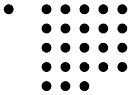
\includegraphics{img/fh-koeln-logo.png}
    \label{logo_fh_köln}
  \end{flushright}
\end{figure}

\begin{center}
\textbf{\Large\newline  Fachhochschule Köln\\
Cologne University of Applied Sciences\\[0.1cm]
\normalsize Campus Gummersbach\\
Fakultät für Informatik und Ingenieurwissenschaften\\[0.5cm]}

 
\Large Verbundstudiengang Wirtschaftsinformatik\\[0.5cm]

\large Masterthesis\\[0.1cm]
  
% Title
{ \huge \bfseries \ Konzepte der Nebenläufigkeit  \\[0.1cm]
        unter Android \\[0.5cm]
        
}
\vfill

\begin{table}[h]
\centering
\begin{tabular}{ll}
  Prüfer:         & Prof. Dr. Erich Ehses \\
  Zeitprüfer:     & Prof. Dr. Frank Victor \\
  vorgelegt am:   & \today \\
  von cand.:      & Stephan Wagner \\
  aus:            & Overath \\
  Telefon-Nr.:    & +49-176-80007570 \\
  Matrikel-Nr.:   & 1106011828 \\
  E-Mail-Adresse: & stephan.wagner.mi738@gmail.com
\end{tabular}
\end{table}
\end{center}
\end{titlepage}



\onehalfspacing % 1,5-facher Zeilenabstand

\chapter*{Zusammenfassung}
In dieser Arbeit werden unterschiedliche Konzepte zur Realisierung von Nebenläufigkeit unter dem Android Betriebssystem untersucht. Nebenläufigkeit stellt einen Entwickler häufig vor große Herausforderungen. Unter Android bestehen dabei noch zusätzliche Besonderheiten an denen sich die hier vorgestellten Konzepte beweisen müssen. Dabei werden diese im Detail an Hand von konkreten Implementierungsbeispielen vorgestellt und analysiert. Im Anschluss fließen die aus der Detailanalyse gewonnenen Ergebnisse in eine Szenarien basierte Analyse um daraus Erkenntnisse für den sinnvollen Einsatz der Konzepte abzuleiten.
fdg \newline
asdfasdf

\tableofcontents
\listoffigures


\chapter{Einleitung}
Applikationen für mobile Endgeräte sind in großer Vielfalt am Markt verfügbar und erfreuen sich quer durch alle Bevölkerungsschichten wachsender Beliebtheit. Dabei nehmen die Möglichkeiten, wie sogenannte Apps den Alltag bereichern und / oder erleichtern mit jeder neuen Hardwareschnittstelle zu. Die meist verbreiteten Betriebsysteme iOS und Android ermöglichen dabei mit dem jeweiligen Software Development Kit (kurz SDK) den Zugriff auf diese Schnittstellen. Applikationsentwickler haben damit die Möglichkeit dem Nutzer ein reichhaltiges Angebot von Applikationen zur Verfügung zu stellen.
\section{Motivation}
Die rasante Verbreitung der Technologien zu Mobilen Geräten erschließt ein großes Potential an Innovationsträgern für neue Applikationen. Da die Android Applikationsentwicklung auf der freien Entwicklung basiert (d.h. Jedem ist es erlaubt Apps zu schreiben), gehören neben dem Kreis professioneller Android Entwickler ebenso nicht professionelle und Einsteiger in der Android Entwicklung zu den Innovationsträgern. Jedoch ist die Einstiegshürde selbst für erfahrene Softwareentwickler unter Umständen so hoch, dass die Umsetzung von neuen Ideen bereits im Ansatz scheitern kann. Um die Komplexität der Entwicklung von Applikationen unter iOS zu reduzieren, stellt der Hersteller Apple zumindest eine Entwicklungsumgebung bereit, in der einfache Funktionalität auf einem Storyboard aus einer Auswahl an Funktionen zusammengestellt werden kann. Kenntnisse in der Programmierung sind somit nicht in allen Entwicklungsschritten zwingend notwendig. Dagegen bietet Android keine vergleichbare Unterstützung durch ein Storyboard, wodurch die Entwicklung von Android- Applikationen zahlreiche, hohe Einstiegshürden birgt. Bei einer Einstiegshürde handelt es sich um die technische Umsetzung von bestimmten Funktionalitäten, die für eine Applikation benötigt werden, was  dazu führen kann, dass ein und dieselbe Funktionalität in unterschiedlichen Applikationen von Entwicklern auf unterschiedliche Art und Weise implementiert wird. Für weniger erfahrene Entwickler oder Einsteiger besteht hier die Gefahr, Funktionalität fehlerhaft oder unperformant zu konzipieren.\newline
Ein weiteres Problem ist das des Code-Copy. Dies beschreibt, wie gleiche Funktionalität durch Kopieren des jeweiligen Sourcecode in unterschiedliche Softwarekomponenten durch Dublizieren des Sourcecode integriert wird, anstatt auf eine zentrale Implementierung zu referenzieren.

\section{Zielsetzung}
Ziel dieser Projektarbeit ist es, einen Lösungsansatz zu entwickeln, um den Problemstellungen in der Android- App- Entwicklung bezüglich der Einstiegshürden und dem Problem des Code-Copy entgegenzuwirken. Hierzu sind mittels Hilfe von konkreten Implementierungsbeispielen die Einstiegshürden sowie die Gefahren des Code-Copy bei der Android-Entwicklung zu veranschaulichen und daraus Erkenntnisse für die Konzeption eines allgemeinen Lösungsansatzes abzuleiten. Dieser Ansatz ist abschließend dahingehend zu untersuchen, ob er für weitere technologische Problemstellungen in diesem Kontext der Android- Entwicklung anwendbar wäre. Die Arbeit, sowie die darin aufgeführten Codebeispiele, beziehen sich auf die Android- Version 4.x. Die Version 4.0 (API Level 14) stellt dabei die Mindestanforderung an das verwendete Betriebssystem dar.

\section{Inhalt und Vorgehen}
Um sich der Problemstellungen in Android bezüglich der Einstiegshürden und dem Code Copy anzunähern, wird dessen konkrete Ausprägung am Beispiel „Steuerung von Funktionalität durch Gesten“ untersucht. Hierzu wird zunächst ein allgemeines Verständnis zu Gesten, sowie deren Erkennung aufgebaut, um dann an Hand von konkreten Bespielen ein tieferes Verständnis der Steuerung von Funktionalität mittels Gesten zu erlangen. Die dabei gewonnenen Erkenntnisse werden in einem Abstraktionsprozess auf eine generische Implementierung übertragen, um weitergehend zu diskutieren, wie diese für andere App Projekte verfügbar gemacht werden kann.\newline
Abschließend steht die Frage, inwieweit der Lösungsansatz valide ist gegenüber weiteren Ausprägungen der Eingangsproblematik, bzw. ob sich daraus sogar ein allgemeines Lösungskonzept ableiten lässt.

\chapter{Gesten im Allgemeinen}
\section{Begriffsdefinition}
Gesten sind bewusste oder unbewusste Bewegungen bzw. Handlungen mit symbolischem Charakter eines Individuums, mit dem Ziel der non- verbalen Kommunikation oder der Unterstützung einer verbalen Kommunikation. Die Art und Weise einer Geste hängt dabei stark von den mentalen Modellen des Individuums ab, die es versucht durch die Geste zum Ausdruck zu bringen. Die Art und Weise der gestikulierenden Bewegung sowie die Semantik dahinter hängt u.a. vom kulturellen Hintergrund des Individuums, aber auch von körperlichen Eigenschaften wie Behinderungen ab. \newline
Spätestens seitdem Dr. Sam Hurst 1974 den ersten Touchscreen entworfen hat, wird bei der Entwicklung technischer Systeme versucht, die Gesten als Interaktionsparadigma zu nutzen, um eine möglichst intuitive Mensch-Computer-Interaktion zu schaffen. Das durch die Gesten zu steuernde System registriert dabei vordefinierte Gesten mittels einer geeigneten Hardwareschnittstelle (z.B. Touchscreen) und führt pro Geste definierte Aktionen aus. In diesem Kontext wird unterschieden zwischen Single- und Multi-Touch-Gesten. Single-Touch-Gesten meinen einzelne Berührungen und Bewegungen (also z.B. mit einem Finger) auf einem Touchscreen. Der Android Style Guide nennt hierzu Gesten wie „Touch“, „Drag“ oder „Swipe and Drag“. Im Gegenzug bilden Multi-Touch-Gesten Bewegungen mit mehreren Fingern ab (siehe hierzu im Android Style Guide „Pinch-Open“ und „Pinch-Close“). Die Entwicklung der Sensoren zur Registrierung der einzelnen Berührungsformen ist dabei entscheidend.

\section{Meilensteine der Sensortechnologie zur Registrierung von Gesten}
Die Entwicklung der Sensortechnologie zur Registrierung von Gesten ist in den letzten Jahren stark vorangetrieben worden. Das IBM Simon (1992) gilt als das erste mobile Endgerät mit Touchscreen. Der Grundstein für die Weiterentwicklung des Touchscreen wurde jedoch bereits in den frühen 70er Jahren gelegt, indem Dr. Sam Hurst das erste transparente Touchdisplay entwickelte. Der darin verbaute Sensor konnte einfache Single-Touch-Gesten registrieren. In den folgenden Jahren wurden die unterschiedlichsten technischen Verfahren entwickelt. Daraus ist 1984 der erste Touchsensor hervorgegangen, mit dem Multi-Touch-Gesten registriert werden konnten. Der Zeitstrahl in Abbildung 1 gibt einen Einblick in eine Auswahl von wichtigen Meilensteinen bei der Entwicklung der Sensortechnologie:
\begin{figure}[H]
  \begin{centering}
    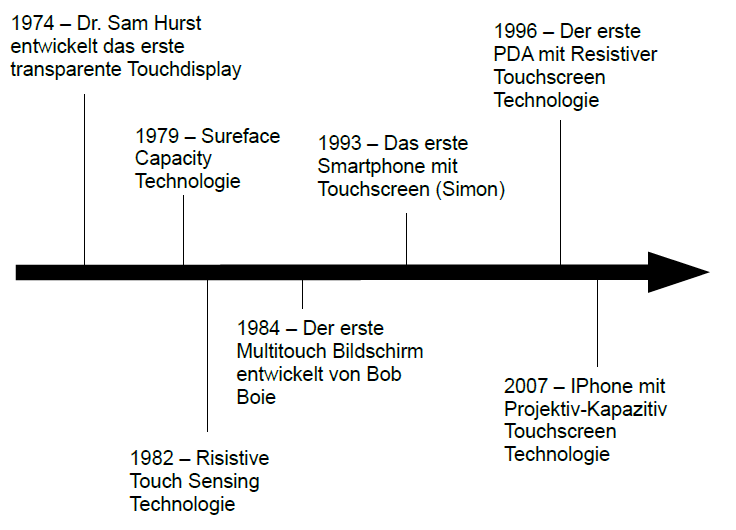
\includegraphics[width=0.8\textwidth]{img/Einleitung_History_Touchscreen.png}
    \caption{Meilensteine der Touchscreenentwicklung \cite[vgl. From touch displays to the Surface]{001}}
    \label{Touchscreenentwicklung_Meilensteine}
  \end{centering}
\end{figure}
Einen kurzen Einblick in die unterschiedlichen Sensortechnologien bietet das folgende Kapitel.

\section{Sensortechnologieen zur Registrierung von Berührungen}
Die Entwicklung der Gesten hängt unmittelbar mit der Entwicklung der Sensortechnologie zur Registrierung von Berührungen auf einem Bildschirm zusammen. Dabei sind die ersten Berührungsbildschirme, basierend auf optischen Bildschirmsensoren, beschränkt auf einfache Druck-Gesten. Diese Technologien sind aus der Entwicklung des Touchscreens hervorgegangen:
\subsection{Biegewelle (Dispersive Signal) Technologie}
\begin{figure}[H]
  \begin{centering}
    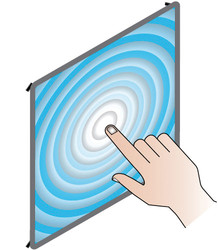
\includegraphics[width=0.8\textwidth]{img/Biegewelle.jpg}
    \caption{Biegewelle Technologie \cite[vgl. DST-Biegewellen]{002}}
    \label{Biegewelle}
  \end{centering}
\end{figure}
Das Funktionsprinzip basiert auf der Ausbreitung von durch Berührung ausgelösten Schwingungen in einem bestimmten Medium, welches in den Bildschirm integriert ist. Diese Schwingungen werden an den Bildschirmek-ken durch Sensoren gemessen. Der relative Zeitunterschied in Bezug zu den Auftreffzeitpunkten der Welle auf die Sensoren wird für die Berechnung der Position der Berührung auf dem Bildschirm verwendet. Diese Technologie leistet nur die einfache Erkennung einer Berührung (z.B. nur ein Finger), da bei mehrfacher Berührung die Überlagerung von Wellen (Interferenz) zu ungenauen Berechnungen der Positionen führen würde.

\subsection{Infrarot- Gitter Technologie}
\begin{figure}[H]
  \begin{centering}
    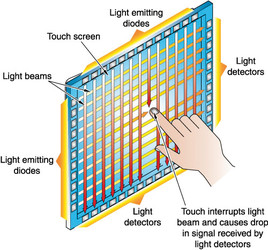
\includegraphics[width=0.8\textwidth]{img/Infrarot_Gitter.jpg}
    \caption{Infrarot Gitter Technologie \cite[vgl. Infrarot-Gitter]{002}}
    \label{Infrarot_Gitter}
  \end{centering}
\end{figure}
Die Infrarot-Gitter-Technologie teilt den Touchbildschirm mittels Infrarotstrahlen in ein Raster auf. Jede Berührungsgeste unterbricht einzelne Infrarotstrahlen, was durch entsprechende Sensoren wahrgenommen wird. Mehrfache Berührungen werden durch dieses Konzept prinzipiell unterstützt, wobei es zu technischen Problemen führen kann, wenn mehrere dicht zusammenliegende Berührungspunkte zu unterscheiden sind, da hierfür die Maschen des Infrarotrasters eng genug konstruiert sein müssen.

\subsection{Optische Rezeptor Technologie}
\begin{figure}[H]
  \begin{centering}
    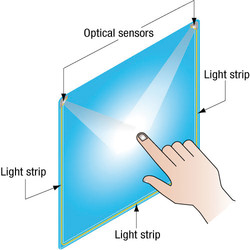
\includegraphics[width=0.8\textwidth]{img/optical_receptor.jpg}
    \caption{Optische Rezeptor Technologie \cite[vgl. Optisch]{002}}
    \label{optical_receptor}
  \end{centering}
\end{figure}
Die optische Rezeptorentechnologie zur Registrierung von Berührungen auf dem Touchbildschirm realisiert die Erkennung von Gesten mittels optischer Sensoren an den Bildschirmecken. Diese messen bei Berührung des Bildschirmes die Lichtunterbrechung des an den Kanten des Bildschirmes emittierten Lichtes. Ähnlich wie bei der Infrarottechnologie gibt es auch hier technologische Schwierigkeiten, dicht zusammenliegende Berührungspunkte auseinanderzuhalten, besonders, da lediglich zwei optische Sensoren verbaut wurden.

\subsection{Resistive Touchbildschirm Technologie}
\begin{figure}[H]
  \begin{centering}
    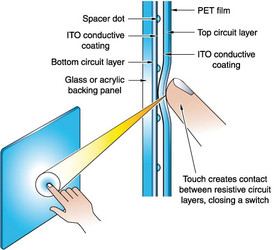
\includegraphics[width=0.8\textwidth]{img/Resistiv.png}
    \caption{Resistive Technologie \cite[vgl. Resistiv-4-5-7-und-8-Draht]{002}}
    \label{Resistiv}
  \end{centering}
\end{figure}
In der resistiven Touchscreen-Technologie wird ein Touchbildschirm in Deckschicht und Grundschicht unterteilt. An den Innenkanten beider Schichten ist ein leitender Film angebracht, der je mit unterschiedlicher Spannung geladen ist. Wie in der Abbildung gezeigt, schließt eine Berührung den Stromkreis und mit Hilfe der an den Bildschirmkanten angebrachten Sensoren die genauen Koordinaten des Berührungspunktes ermittelt. Prinzipiell ist bei dieser Technologie die Erkennung von Mehrfachberührungen möglich, jedoch hängt dies von den verbauten Sensoren ab.

\subsection{Surface Accustic Wave (SAW)}
\begin{figure}[H]
  \begin{centering}
    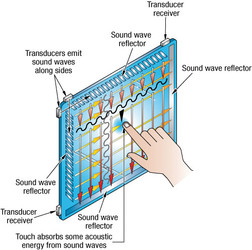
\includegraphics[width=0.8\textwidth]{img/surface_accustic_wave.png}
    \caption{Surface Accustic Wave Technologie \cite[vgl. Surface-Acoustic-Wave-Saw]{002}}
    \label{surface_accustic_wave}
  \end{centering}
\end{figure}
Das technische Prinzip dieser Technologie ist vergleichbar mit dem des Infrarot-Gitters. Schallwellen werden an bestimmten Punkten des Touchbildschirms emittiert und an zwei Kanten (x;y) so reflektiert, dass ein Raster durch die Schallwellen im Berührungsbereich aufgespannt wird. An den zwei übrigen Kanten leiten Reflektoren die einzelnen Schallwellen zu einem Sensor. Die Berührung hat eine Dämpfung der Schallwellen (in x- und y-Richtung) zur Folge, die zum Zeitpunkt der Berührung den Berührungspunkt passieren. Da die Schallwellen zeitverzögert erzeugt werden, also nur immer eine Schallwelle in eine X-Richtung und nur eine in Y-Richtung, ist somit der Berührungspunkt genau zu ermitteln. Dies bedeutet jedoch auch, dass zum selben Zeitpunkt nur ein Berührungspunkt ermittelbar ist, womit Multi-Touch-Gesten durch diese Technologie nicht unterstützt werden.

\subsection{Oberflächen-kapazitive Touchscreen Technologie}
\begin{figure}[H]
  \begin{centering}
    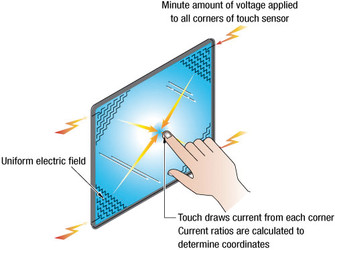
\includegraphics[width=0.8\textwidth]{img/oberflaechen_kapazitiv.png}
    \caption{Oberflächen Kapazitive Technologie}
    \label{oberflächen_kapazitiv}
  \end{centering}
\end{figure}
Die kapazitive Touchscreen-Technologie registriert Berührungen durch die Ablenkung innerhalb eines elektronischen Feldes, welches durch Elektroden an den Bildschirmkanten erzeugt wird. Sensoren an den Bildschirm-ecken messen dabei das elektronische Feld und damit jegliche durch Berührung ausgelöste Veränderung des Feldes. Der Finger fungiert dabei als Erdung, über den Elektronen aus dem Feld abfließen und somit für einen Spannungsabfall während der Berührung sorgt. Die genaue X- und Y- Koordinate errechnet sich aus den Strömen, die an den Sensoren registriert werden. Auch hier beschränkt sich die Technologie auf die Registrierung von lediglich einer Geste.


\subsection{Projiziert Kapazitiver Touchscreen Technologie}
\begin{figure}[H]
  \begin{centering}
    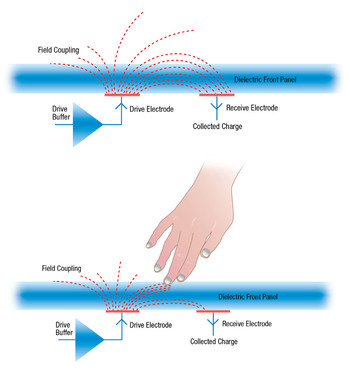
\includegraphics[width=0.8\textwidth]{img/projiziert_kapazitiv.png}
    \caption{Projiziert Kapazitive Technologie \cite[vgl. Projected-Capacitive]{002}}
    \label{projiziert_kapazitiv}
  \end{centering}
\end{figure}
Die projiziert- kapazitive Touchscreen-Technologie erweitert die Oberflächen-Kapazitiv-Technologie um einzelne kleinere Felder auf dem Touchbildschirm und ist die aktuellste der genannten Technologien. Der wesentliche Vorteil gegenüber der Oberflächen-Kapazitiven-Technologie ist, dass hier schon die Näherung eines Fingers ausreicht, um eine Berührung zu registrieren. Dadurch ist es möglich selbst durch dünne Handschuhe eine Berührung zu registrieren, was einen klassischen Einsatzkontext für den medizinischen Bereich darstellt. Die Abbildung zeigt, wie allein durch die Annäherung eines Fingers Teilbereiche des Feldes durch natürliche Ladung in den Fingern abgelenkt werden.

\chapter{Gestenerkennung und Steuerung von Funktionalität durch Gesten}
\section{Signalverarbeitung und erste Gesteninterpretation durch das Android OS}
Die Auflistung der einzelnen Technologien zum Touchbildschirm hat gezeigt, wie unterschiedlich die Umsetzungen der Berührungserkennung und deren Leistungsfähigkeit in Bezug auf die Erkennung von einfachen und mehrfachen Berührungen zur selben Zeit sind. Das Android Betriebssystem ist darauf ausgelegt, die unterschiedlichen Formen von Touchbildschirmen zu unterstützen. Je nach verbauter Technologie ist dabei die Erkennung von mehreren Berührungspunkten freigeschaltet oder nicht. Für den Entwickler einer Android Applikation ist dies jedoch völlig transparent. Im Falle einer registrierten Berührung wirft die API ein sogenanntes „MotionEvent“. Die Android API leistet hier eine erste Interpretation der Gesten, denn je nach Art der Berührung wird ein bestimmtes „MotionEvent“ gefeuert. Diese Events können abgefangen werden und liefern Berührungsparameter (Koordinaten) für eine weitere, detailliertere Interpretation der Gesten.
Der folgende Abschnitt beschreibt die prototypische Implementierung exemplarischer Gesten und geht neben den Besonderheiten und Schwierigkeiten der Gesteninterpretation auch auf die durch die Android API angebotenen MotionEvents ein.


\section{Erkennung und Interpretation von Gesten sowie Steuerung jeweiliger Funktionalität durch Gesten}
Für die Erkennung von Gesten bietet das Android SDK die Schnittstelle OnTouchListener an. Darin lässt sich die Methode\newline
   \centerline{ \texttt{boolean onTouch(View zoomView, MotionEvent anEvent)\{...\}}}\newline
überschreiben. Über den Parameter anEvent vom Typ MotionEvent können unterschiedliche Berührungsgesten erkannt werden. Die Methode OnTouchListener wird in Abhängigkeit von bestimmten Ereignissen aufgerufen. Hierzu ist zu einer View-Instanz die konkrete Implementierung des OnTouchListener Interfaces zu adressieren:\newline \centerline{\texttt{viewInstance.setOnTouchListener(touchListenerImpl);}}\newline
Wenn der Touchsensor eine Berührung registriert, wird für das jeweilige Layout geprüft, welche darin enthaltenen Views die Methoden des OnTouchListeners überschreiben und das Event an die jeweilige Implementierung weitergeleitet. Des Weiteren ist dem Objekt vom Typ MotionEvent zu entnehmen, um welche Art von Berührung es sich handelt.
Je nach Art und Weise der Berührung liefert die Maskierung der zur Event Aktion\newline
\centerline{\texttt{anEvent.getActionMasked()}}\newline\newline
ein Ergebnis, welches durch ein Element der Menge aus den folgenden Konstanten beschrieben wird:\newline
Menge M\newline
\{\newline\texttt{
   int ACTION\_DOWN = 0;\newline
   int ACTION\_UP = 1;\newline
   int ACTION\_MOVE = 2;\newline
   int ACTION\_CANCEL = 3;\newline
   int ACTION\_OUTSIDE = 4;\newline
   int ACTION\_POINTER\_DOWN = 5;\newline
   int ACTION\_POINTER\_UP = 6;\newline
   int ACTION\_HOVER\_MOVE = 7;\newline
   int ACTION\_SCROLL = 8;\newline
   int ACTION\_HOVER\_ENTER = 9;\newline
   int ACTION\_HOVER\_EXIT = 10;\newline}
\}\newline \newline
Für die Interpretation der Gesten und weiter die Steuerung exemplarischer Funktionalitäten wie Zoom oder Drag gilt dann:\newline\newline
ACTION\_DOWN: Der Touchsensor registriert eine Berührung in einem in sich geschlossenen Bereich.\newline
Beispiel: Die Fingerkuppe eines Nutzers berührt den Touchscreen. Die Koordinaten erhält der Entwickler durch das Auslesen des Event-Parameters. Über die Methoden\newline
\centerline{\texttt{anEvent.getX()} und}  \newline
\centerline{\texttt{anEvent.getY()}}\newline
können die Koordinaten ausgelesen werden, auf denen sich ein Finger auf dem Touchbildschirm befindet. Diese Methoden geben im Fall von mehrerer Berührungen (z.B. mehrere Finger) immer die Koordinaten des ersten Berührungspunktes an.\newline\newline
ACTION\_UP: Der Touchsensor registriert das Aufheben einer ursprünglich registrierten Berührung. Dies setzt zuvor die Registrierung einer ACTION\_DOWN voraus.\newline\newline
ACTION\_POINTER\_DOWN:
Der Touchsensor registriert eine zweite Berührung (zweiter Finger). Die Koordinaten der zweiten Berührung, sowie auch im Falle weiterer Berührungspunkte, lassen sich aus dem Event entsprechend der Reihenfolge der Berührung ermitteln:
\centerline{\texttt{anEvent.getX(0..n);}}\newline
\centerline{\texttt{anEvent.getY(0..n);}}\newline
Dies entspricht der Berührung mit dem ersten bis N-ten Finger. Für die Funktionalität Zoom ist es notwendig, die initiale Distanz zwischen den zwei Berührungspunkten zu ermitteln und temporär vorzuhalten.\newline\newline
ACTION\_MOVE: Der Touchsensor registriert eine Bewegung weg vom ursprünglich registrierten Berührungspunkt, dessen Ermittlung diesem Event vorausgeht. Um die o.g. Funktionalitäten zu realisieren, wird für die Ein-Finger-Geste "Drag" der Richtungsvektor bei einer Bewegung auf dem Touchbildschirm ermittelt, indem vom initialen Berührungsspunkt bis zur aktuellen Position des Fingers die Differenz in x wie in y Richtung errechnet wird.


\section{Gestengesteuertes Vergrößern und Verkleinern sowie Veränderung des Fokus für Darstellungsobjekte vom Typ ImageView}
Ian F. Darwin liefert mit seinem Kochbuch für die Android Entwicklung zu der Zoomfunktionalität folgenden Ansatz: \newline
\texttt{// Remember some things for zooming \newline
PointF start = new PointF();\newline\newline
ImageView view = (ImageView) v;\newline
// make the image scalable as a matrix \newline
view.setScaleType(ImageView.ScaleType.MATRIX);\newline
...\newline
switch (event.getAction() \& MotionEvent.ACTION\_MASK) \{ \newline
case MotionEvent.ACTION\_DOWN: //first finger down only\newline
start.set(event.getX(), event.getY());\newline
break;\newline
...\newline
case MotionEvent.ACTION\_MOVE:\newline
if (mode == DRAG)\newline
matrix.postTranslate(event.getX() - start.x, event.getY() - start.y);\newline
\newline
else if (mode == ZOOM)\newline
matrix.postScale(scale, scale, mid.x, mid.y);\newline
\newline
// Perform the transformation\newline
view.setImageMatrix(matrix);\newline
\} \newline 
}\cite[S. 234-237.]{003}\newline
Diese Auszüge aus Darwins Kochbuch zur Andorid Entwicklung zeigen schematisch die dynamische Skalierung einer ImageView in Abhängigkeit der erkannten Gesten mit Hilfe einer speziell für diesen Objekttyp anpassbaren Matrix. Die Matrix lässt sich direkt aus einer Objektinstanz vom Typ ImageView holen und mittels der Methoden
\begin{itemize}
\item \texttt{postTranslate()} und
\item \texttt{postScale()}
\end{itemize}
verarbeiten. Dabei ist zu beachten, dass die Matrix nicht direkt verändert werden darf, sondern nur deren Kopie. Der Richtungsvektor für die neue Fokussierung und damit Transformation der Matix errechnet sich aus der Differenz der aktuellen Koordinaten zu den Anfangskoordinaten und wird zur Transformation der Matrix entsprechend übergeben:\newline
\centerline{ \texttt{ matrix.postTranslate(event.getX() - start.x,}} \newline \centerline{ \texttt{ event.getY() - start.y) }}\newline \newline
Im Fall von mehreren registrierten Berührungen, wie z.B. bei der Pinch-Open-Geste für die Ansteuerung einer Zoom-Funktionalität, muss zunächst die Anfangsdistanz zwischen den Berührungspunkten auf dem Touchbildschirm ermittelt werden. In einem Koordinatensystem aus zwei Dimensionen (x|y) wird die Länge einer Strecke von P1(xp1|yp1) und P2(xp2|yp2) wie folgt berechnet:
\centerline{$\sqrt{(x_{0}-x_{1})^{2}+(y_{0}-y_{1})^{2}}$ }\newline\newline
In Darwins Implementierung ist dies in der Methode \texttt{spacing()} realisiert. Weiter ist über das gesamte ACTION\_MOVE Event hinweg, die neue Distanz der Berührungspunkte zu berechnen und mit der initialen Distanz in ein Verhältnis zu setzen. Der Quotient aus
\centerline{$ ScaleFaktor = \dfrac{dist_{new}}{dist_{old}}$} \newline\newline
ergibt den Faktor für die Skalierung der ImageView. Die ImageView wird daraufhin entsprechend relativ zu der Positionsänderung der Berührungspunkte neu skaliert.\newline
\centerline{ \texttt{ matrix.postScale(scale, scale, mid.x, mid.y);}} \newline\newline
Darwins Vorgehensweise stellt eine komfortable und einfache Möglichkeit dar, eine ImageView Instanz dynamisch zu skalieren oder den Fokus der Darstellung zu verändern. Jedoch bezieht sich die Lösung allein auf Darstellungselemente vom Typ ImageView, wohingegen die Superklasse View, die durch ImageView erweitert wird, es nicht vorsieht die Matrix zur Skalierung und Positionierung der View direkt zu verändern. Damit ist Darwins Lösung allein für Darstellungsobjekte vom Typ ImageView geeignet.

\section{Abstraktion gestengesteuerter Funktionalitäten zum Skalieren und Fokussieren von Darstellungselementen}
Dieser Abschnitt beschäftigt sich mit der Frage, inwieweit sich der Ansatz von Darwin generalisieren lässt und somit unabhängiger vom Typ des Darstellungsobjektes wird. Kann hierzu eine Lösung gefunden werden, so ist weitergehend zu diskutieren, inwieweit diese für andere Android App Projekte verfügbar gemacht werden kann.

\subsection{Generalisierung der Funktionalitäten zum Skalieren und Fokussieren von Darstellungselementen}
Die skizzierte Implementierung nach I.F. Darwin im letzten Abschnitt zeigt zwar, wie ein bestimmtes Darstellungselement in Abhängigkeit von bestimmten Gesten skaliert, jedoch gilt diese Lösung nicht für andere Darstellungselemente. Ein generischer Ansatz müsste die Skalierung und Fokussierung für alle Darstellungselemente leisten, mindestens jedoch für alle Elemente, die vom Typ android.view.View ableiten.\newline
Der im Folgenden skizzierte Prototyp soll Darwins Ansatz um eine dynamische Anzahl von Darstellungselementen mit der Kompatibilität zu unterschiedlichen Darstellungstypen erweitern.
Dieser Projektarbeit liegt eine prototypische Implementierung bei (Klasse \texttt{Touch.java}), in der das Skalieren und Fokussieren von Darstellungselementen für allgemein alle Objekte ermöglicht wird, die vom Typ \texttt{android.view.View} ableiten (z.B. \texttt{TextView extends View}). Ein entsprechender Algorithmus könnte damit die Funktionalität zur Skalierung und Fokussierung applikationsübergreifend generalisieren. 
Für die Skalierung eines Darstellungsobjektes vom Typ View bietet die Android API folgende Methoden an:
\begin{itemize}
\item \texttt{setScaleX()}
\item \texttt{setScaleY()}
\end{itemize}
und für die Veränderung des Fokus auf die View:
\begin{itemize}
\item \texttt{setTranslationX()}
\item \texttt{setTranslationY()}
\end{itemize}
Ein dabei auftretendes Problem sind unerwünschte Seiteneffekte bei der Verwendung des Listeners zur Registrierung von Berührungen und Bewegungen. Dieser Listener kann einer View zugeordnet werden:
\centerline{\texttt{viewInstance.setOnTouchListener(touchListenerInstance)}}\newline \newline
Wird jedoch dieselbe View-Instanz innerhalb der TouchListener-Implementierung neu skaliert, kommt es auf Grund der angestoßenen Zoom-Funktionalität zu einem flackernden Übergang von der ursprünglichen Skalierung in die neue Skalierung. Dies liegt daran, dass das Koordinatensystem der View durch die Skalierung unmittelbar selbst verändert wird. Stellt diese View jedoch auch das Koordinatensystem für die Gestenerkennung, (\texttt{viewInstance.setOnTouchListener(...)}), so wird die Berechnung des Zoomfaktors gestört.
 \newline
Die View, welche durch den Zoom neu skaliert wird, darf also im Falle einer gestengetriebenen Zoom-Funktionalität nie die Bemessungsgrundlage (Koordinaten) für die Berechnung des Skalierungsfaktors sein. Alternativ kann die sogenannte Parent-View der zu skalierenden View-Instanz als Bemessungsgrundlage herangezogen werden, wie es die folgende Abbildung zeigt: \newline
\begin{figure}[H]
  \begin{centering}
    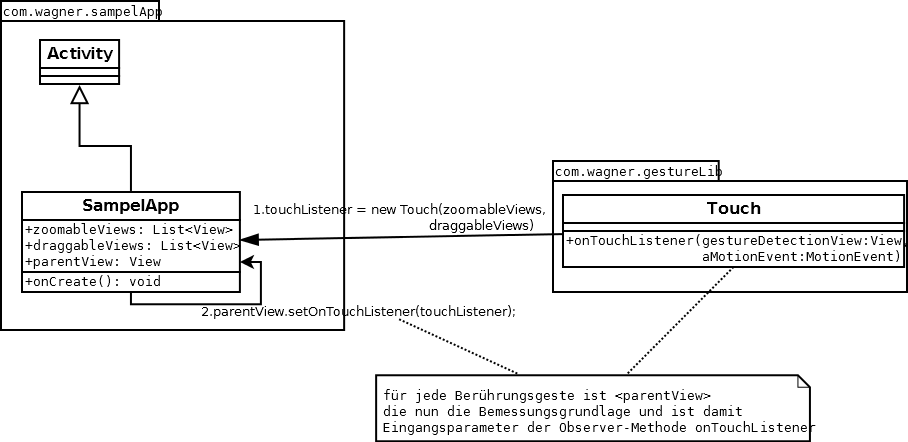
\includegraphics[width=0.8\textwidth]{img/touchFragments.png}
    \caption{Konzeption eines generischen Touchlisteners}
    \label{callingTouchListener}
  \end{centering}
\end{figure} Die Parent-View ist in der Baumstruktur des Layouts einer View- Instanz übergeordnet. 

\subsection{Ausblick zur Integration der generischen Implementierung zu gestengesteuerten Funktionalitäten}
Der letzte Abschnitt hat gezeigt, wie gestengesteuerte Funktionalitäten zum Skalieren und Fokussieren von Darstellungselementen, allgemein für unterschiedliche Darstellungstypen definiert werden können. Dieser Abschnitt gibt einen Ausblick, wie der entworfene Ansatz aus dem letzten Kapitel allgemein für Android Applikationsprojekte angeboten werden kann.\newline
In Android Projekten lassen sich wie auch in anderen Java Projekten zusätzliche Bibliotheken in Form von .jar - Archiv Dateien einbinden. Grundsätzlich ist es möglich diese Bibliotheken manuell in die jeweilige Entwicklungsumgebung einzufügen. Sollten jedoch unterschiedliche Versionen zu den jeweiligen Android APIs unterschieden werden sind bestimmte Werkzeuge zur Versionverwaltung und dem übersichtlichen Management von Abhängigkeiten zu empfehlen. Auch wenn Tests zu Funktionalitäten der Bibliothek vor dem Erzeugen des .jar - Archives durchlaufen werden müssen, sollte dies automatisiert sein. Hierzu gibt es unterschiedliche Werkzeuge, die sich für das Auflösen von Abhängigkeiten sowie das finale Bauen der Applikation anbieten. Exemplarisch bietet sich hier das Build Werkzeug \glqq Maven\grqq mit dem Android Plugin an. Der im letzten Kapitel entworfene Ansatz lässt sich damit in eine eigenständige Bibliothek auslagern, um diesen in unterschiedlichen Android-Applikationsprojekten zu nutzen.

\section{Fazit}
Eingangs stand die Frage im Raum, wie den Einstiegshürden in der Android-Entwicklung sowie dem Problem des Code-Copy entgegen gewirkt werden kann. Anhand der Entwicklung von gestengesteuerter Funktionalität (speziell hier Zoom und Drag) ist verdeutlicht worden, welche Schwierigkeiten auf Einsteiger in der Android Entwicklung warten. Gleichzeitig wird mit der Implementierung nach Darwin (Kapitel 3.3) deutlich, welche Mengen an komplexem Sourcecode zu gestengesteuerter  Funktionalität (siehe Implementierung nach F.Darwin Kapitel 3.3) in Applikationsprojekte integriert werden müsste, um grundlegendes Verhalten zu definieren. Der in diesem Projekt geschaffene Ansatz zur Generalisierung von gestengesteuerter Funktionalität bietet die Möglichkeit den dahinterstehenden Programmcode zu zentralisieren, also Code Copy vorzubeugen und gleichzeitig die Android App-Entwicklung zu vereinfachen.
Für weitere gestengesteuerte Funktionalitäten kann ähnlich verfahren werden, vorausgesetzt es kann ein geeigneter Abstraktionsgrad gefunden werden, wie er hier für die Skalierung und Fokussierung definiert ist.

\bibliography{Praxisprojekt}{}
\bibliographystyle{jureco} %% jurabib, jureco, jurunsrt, 
%% \printindex

\appendix

\chapter*{Anhang}
 \lstinputlisting
    [caption={Die Klasse Touch.java}
       \label{lst:javaclass},
       captionpos=t,language=JAVA]
 {listings/Touch.java}
\addcontentsline{toc}{chapter}{Anhang}
\chapter{Erklärung}

Ich versichere, die von mir vorgelegte Arbeit selbständig verfasst zu
haben. Alle Stellen, die wörtlich oder sinngemäß aus veröffentlichten
oder nicht veröffentlichten Arbeiten anderer entnommen sind, habe ich
als entnommen kenntlich gemacht. Sämtliche Quellen und Hilfsmittel,
die ich für die Arbeit benutzt habe, sind angegeben. Die Arbeit hat
mit gleichem Inhalt bzw. in wesentlichen Teilen noch keiner anderen
Prüfungsbehörde vorgelegen.

\bigskip

Gummersbach, den \today

\bigskip

\bigskip

\bigskip

\bigskip

\bigskip

\bigskip

(Unterschrift)

\end{document}

%% end of file
